\documentclass[a4paper, twoside, 10pt]{report}

\usepackage{fancyhdr}
\usepackage{color}
\usepackage{afterpage}
\usepackage{graphicx}
\usepackage{amsmath, amsfonts, amssymb}
\usepackage[ddmmyyyy]{datetime}
\renewcommand{\dateseparator}{.}
\usepackage{setspace}
\usepackage{titlesec}
\usepackage{tikz}
\usetikzlibrary{calc}
\usepackage[margin=5cm]{geometry}
\usepackage{avant}
\usepackage{makecell}
\usepackage[english]{babel}
\usepackage{wrapfig}
\usepackage{ragged2e}
\usepackage{pgfplots}

\setstretch{1.3}
\setlength{\parskip}{1em}

\titleformat{\chapter}
	{\normalfont\huge\bfseries}{\thechapter}{1em}{}
\titlespacing*{\chapter}{0pt}{3.5ex plus 1ex minus .2ex}{2.3ex plus .2ex}

\AtEndDocument{\cleardoublepage}

\title{Bachelor thesis booklet}
\author{Johannes C. Mayer}
\date{\today}

\newcommand\blankpage{\null\thispagestyle{empty}\addtocounter{page}{0}\newpage}

\renewcommand{\familydefault}{\sfdefault}

\pagestyle{fancyplain}
%\fancyhf{}
\fancyfoot{}
\fancyfoot[le,ro]{{\small \thepage} \\[4mm] }%{\scriptsize Johannes C. Mayer}}

\usepackage[list=true]{subcaption}
\usepackage{tocloft}
\setcounter{lofdepth}{2}
\makeatletter
\newcommand{\figsourcefont}{\footnotesize}
\newcommand{\figsource}[1]{%
  \addtocontents{lof}{%
    {\leftskip\cftfigindent
     \advance\leftskip\cftfignumwidth
     \rightskip\@tocrmarg
     \figsourcefont#1\protect\par}%
  }%
 }
\makeatother

% HOW TO USE ^^^^
%\begin{figure}[hbt]
%\centering
% {\caption{Caption}
%    \figsource{Source}}
%       \subcaptionbox{Caption1}
%{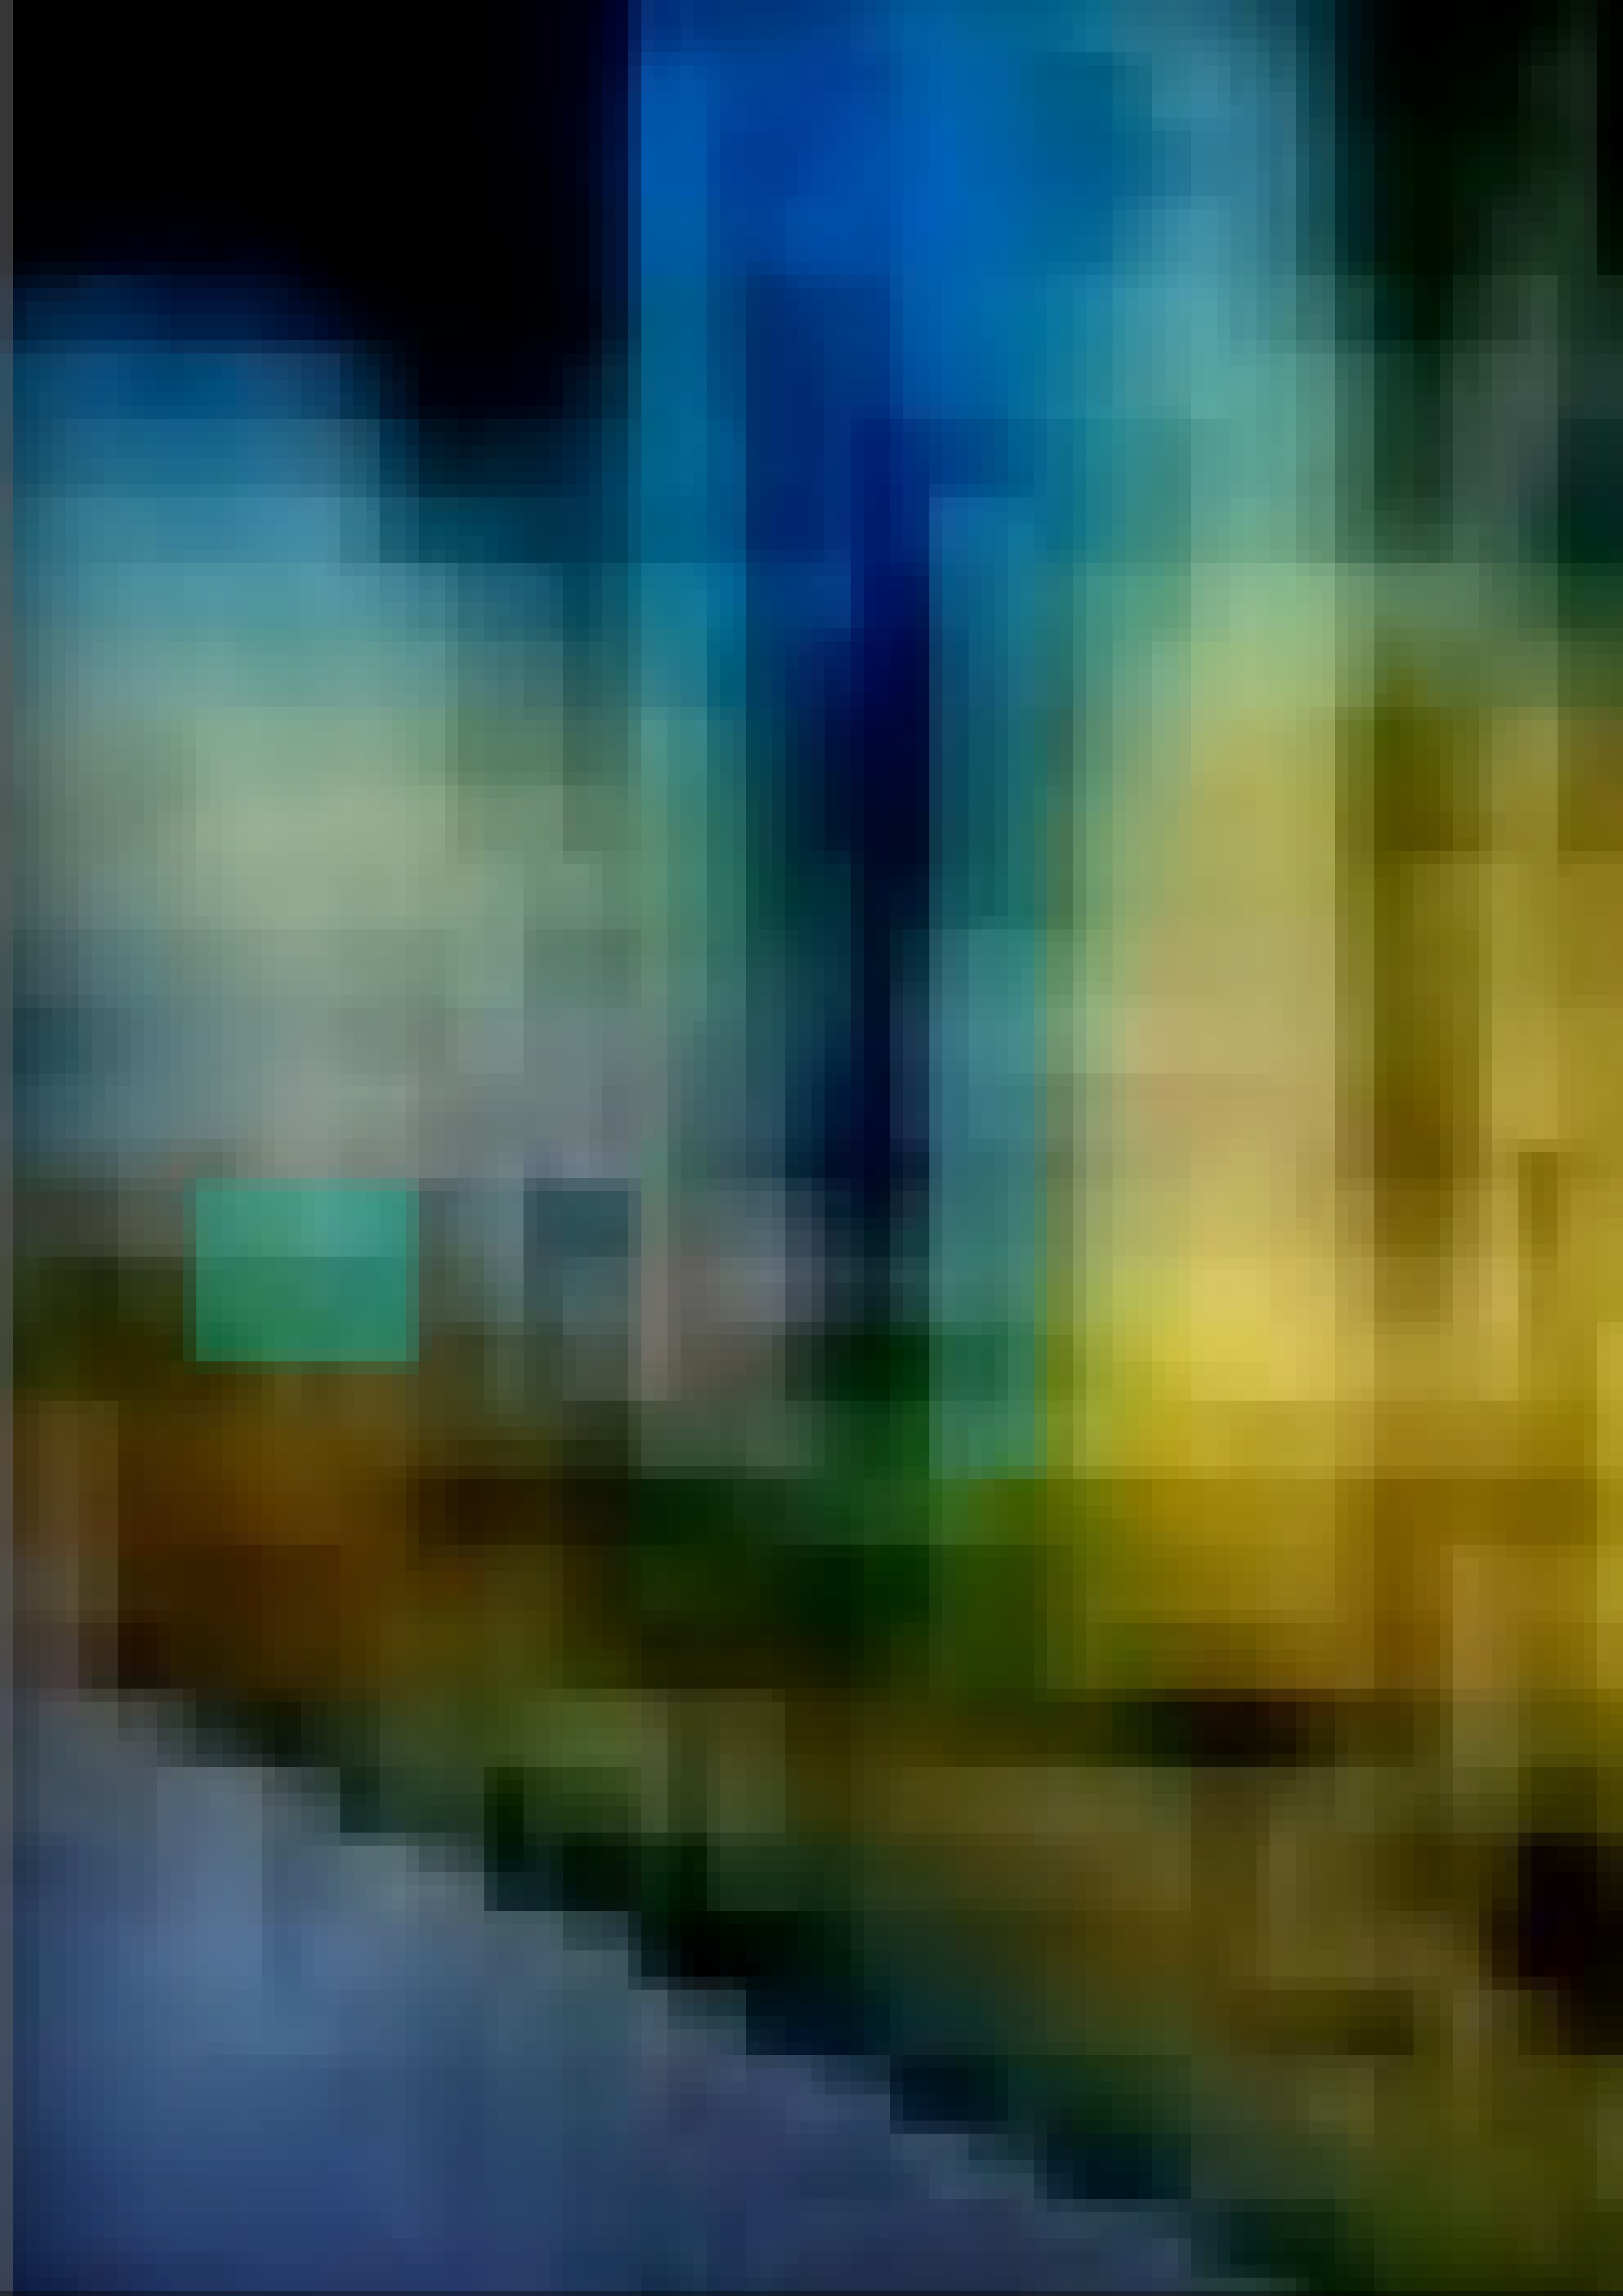
\includegraphics[width=0.4\textwidth]{Images/FrontCover.png}}
%       \figsource{Source1}
%\subcaptionbox{Caption2}
%{ 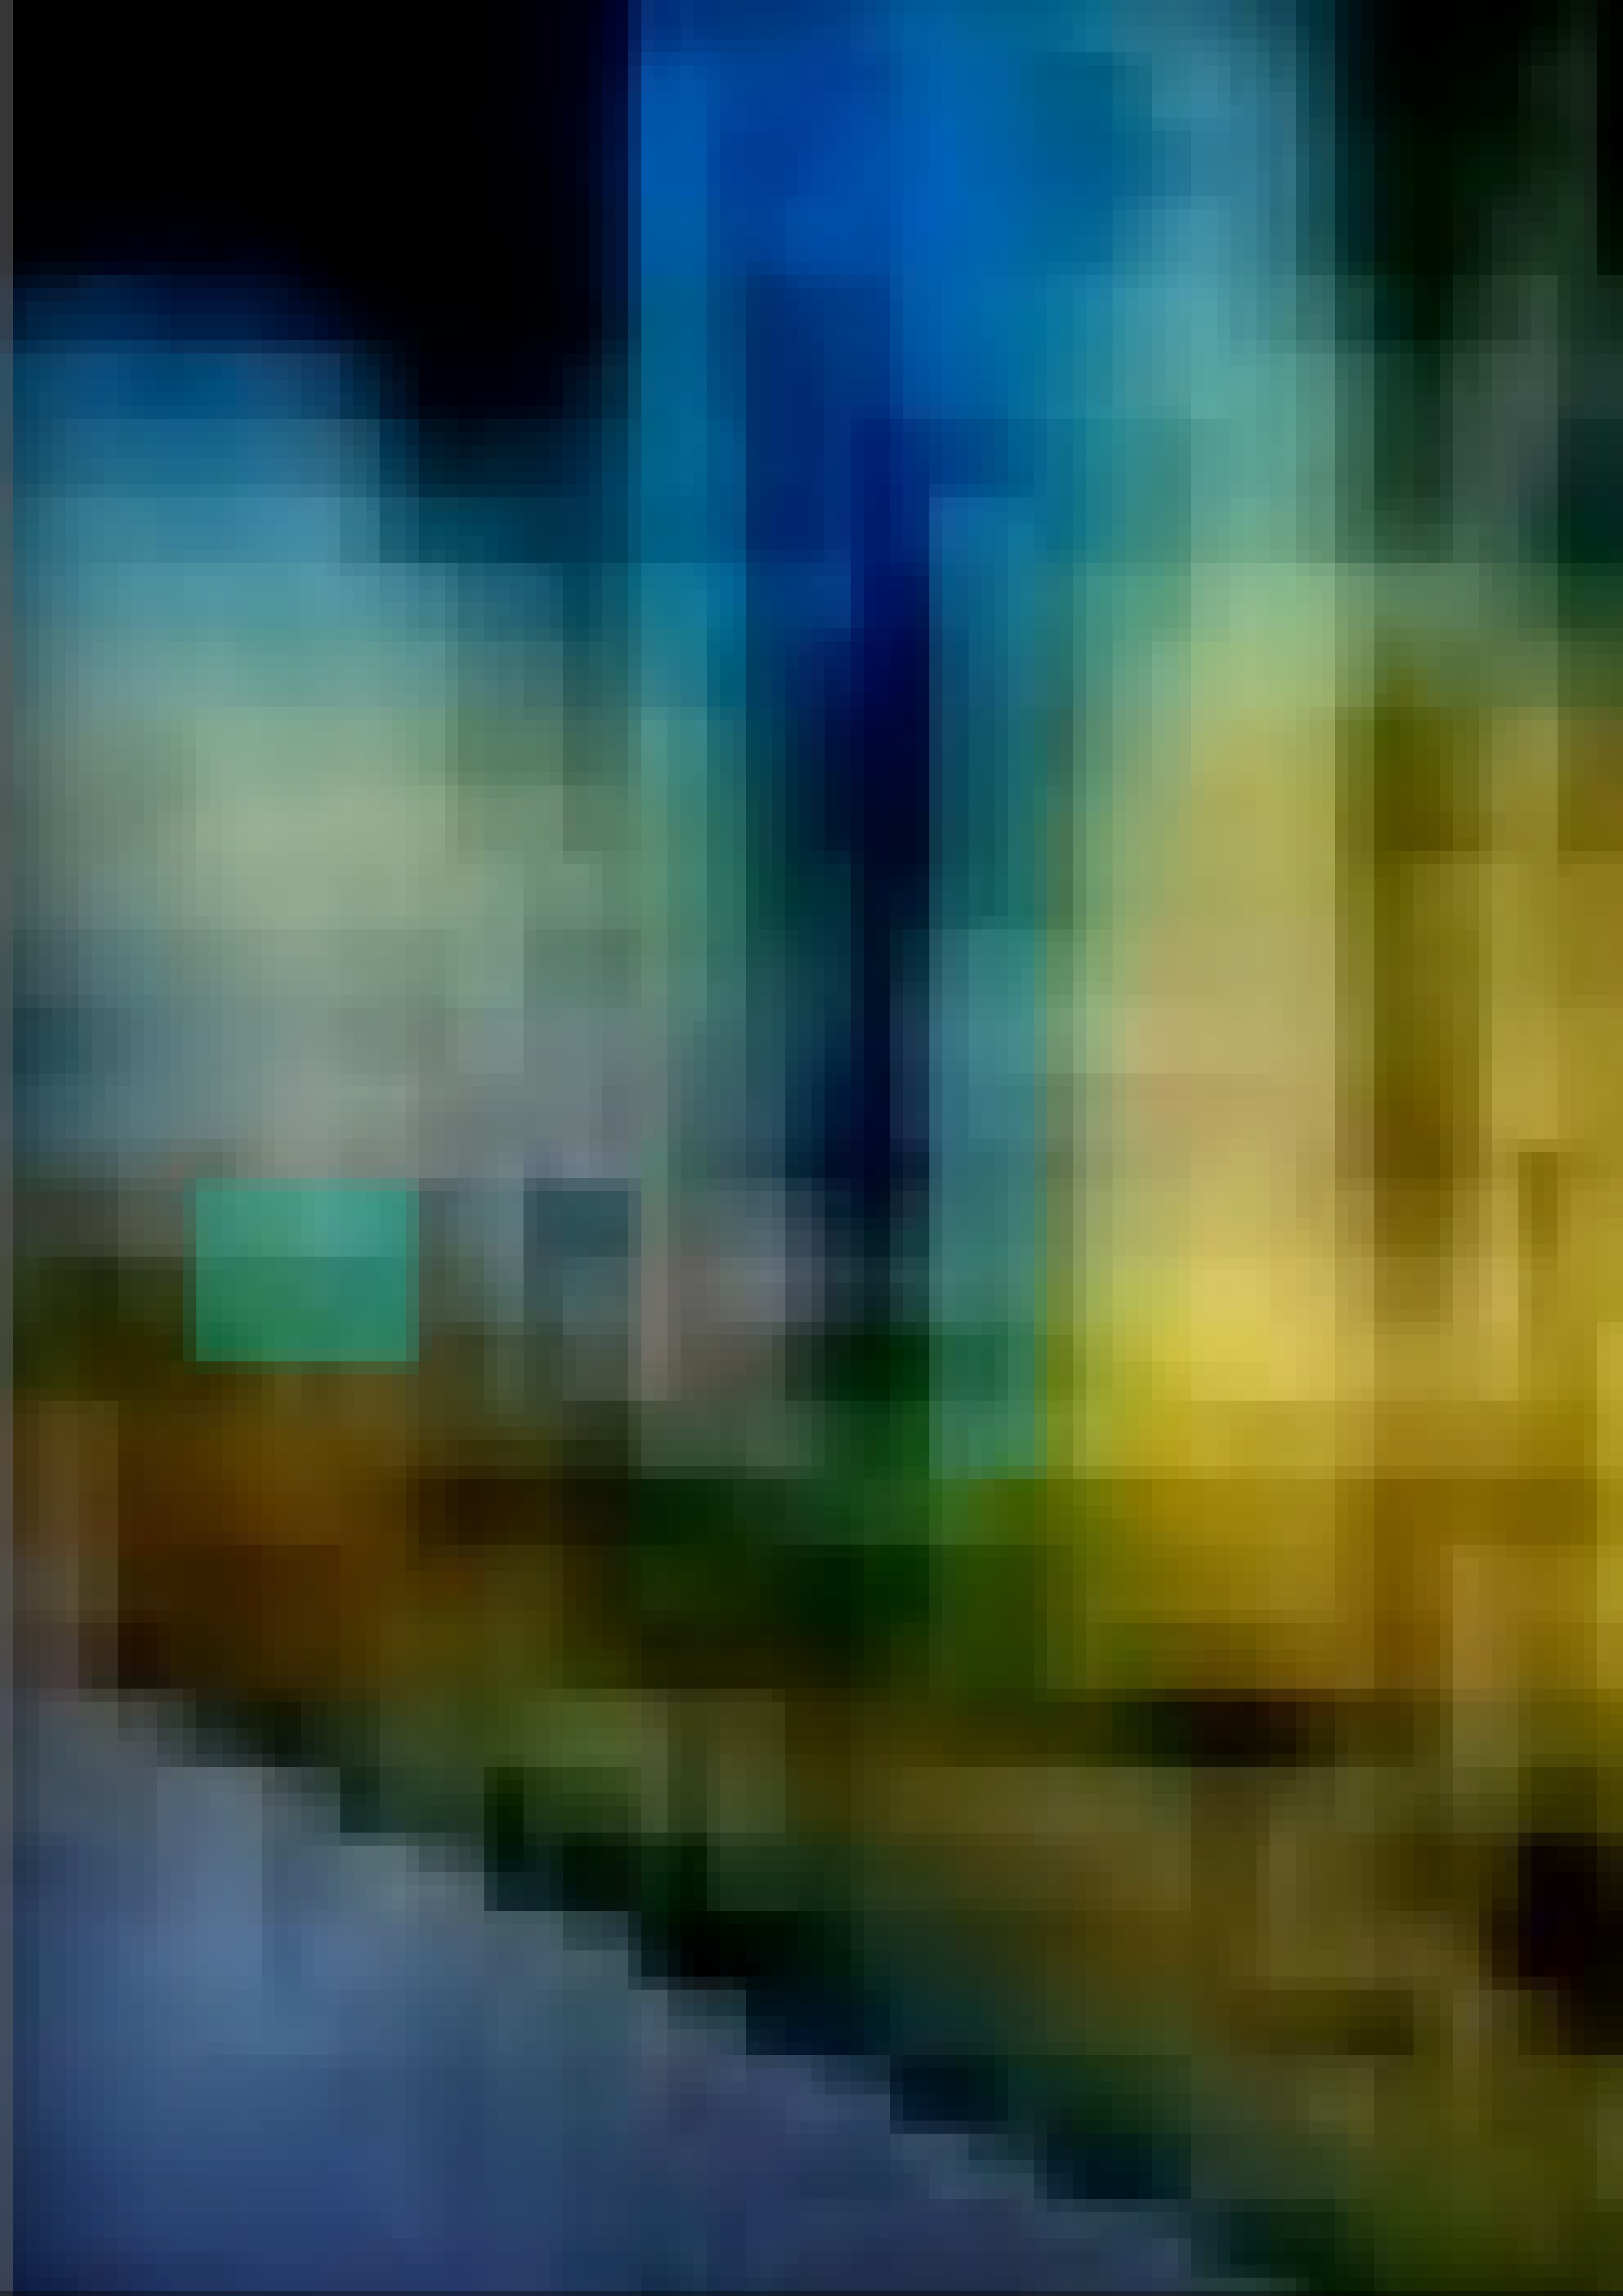
\includegraphics[width=0.4\textwidth]{Images/FrontCover.png}}
%        \figsource{Source2}
%\end{figure}

\begin{document}

\begin{titlepage}
\begin{tikzpicture}[remember picture,overlay]
\node[inner sep=0pt] (background) at (current page.center) {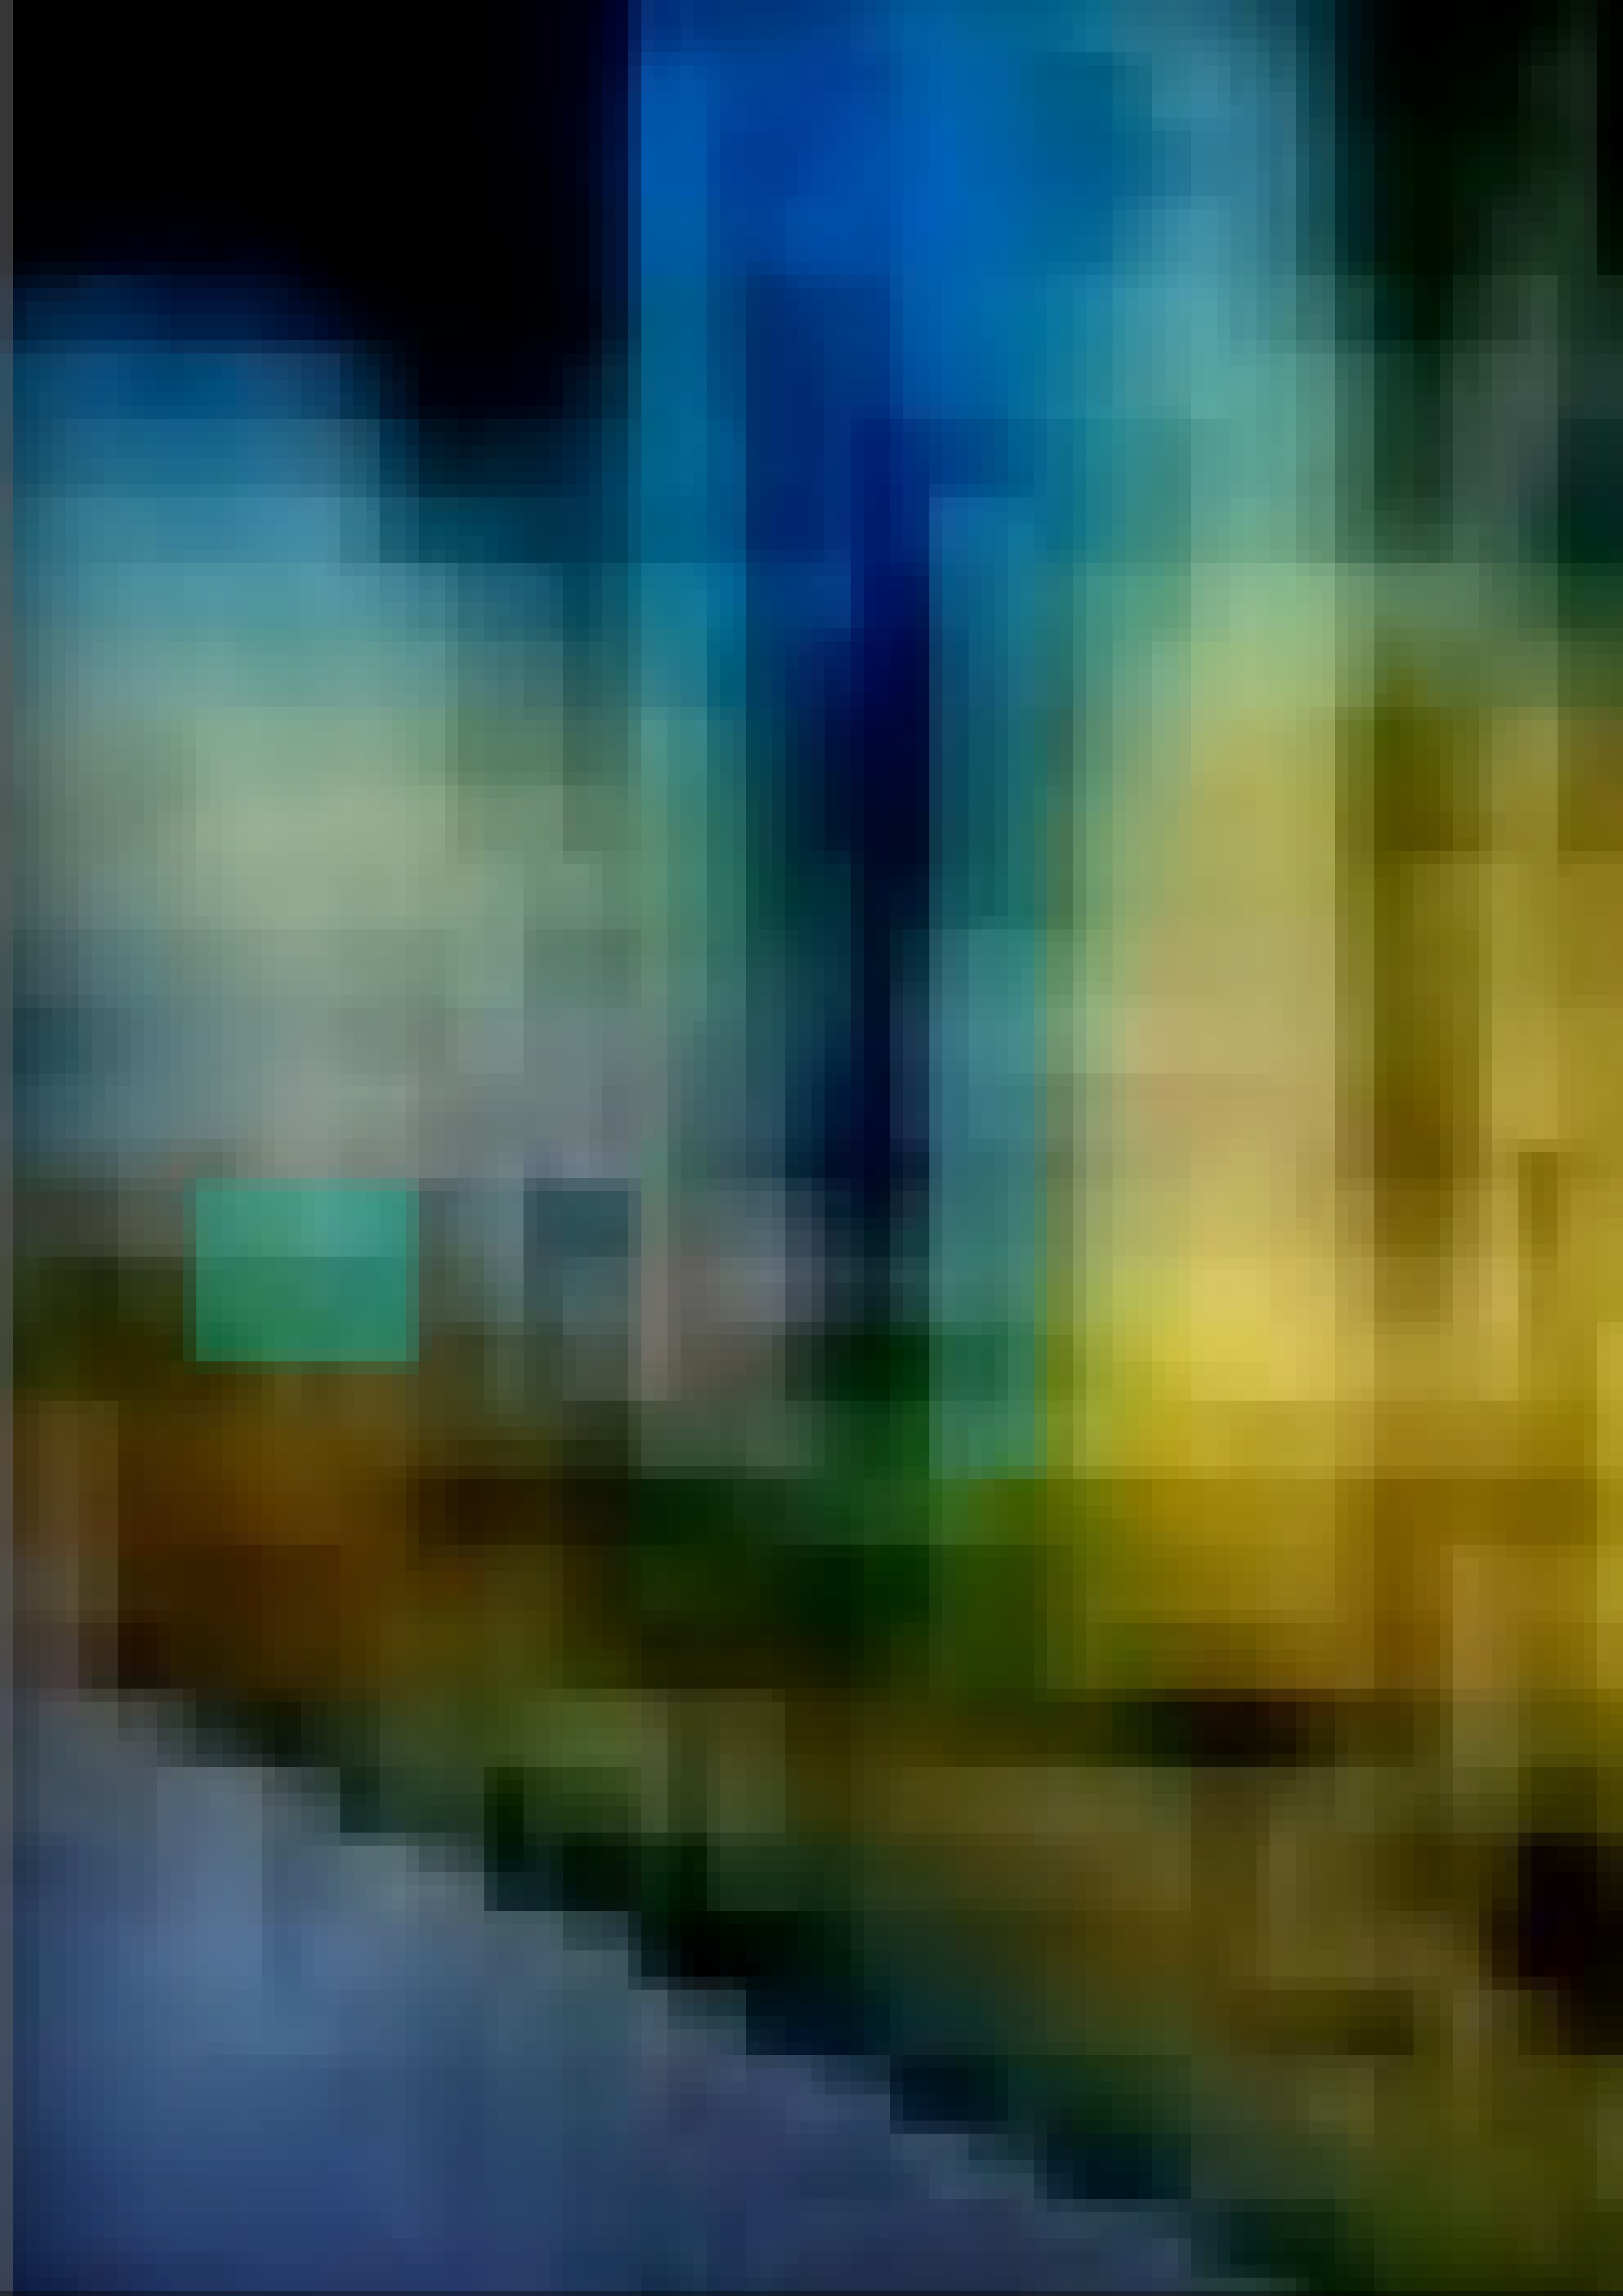
\includegraphics[width=\paperwidth]{Images/FrontCover.png}};
\draw ($(current page.south)+(0,5)$) node [fill=black,fill opacity=0.6,text opacity=1,inner sep=1cm]{\color{white}\Huge\centering\bfseries\sffamily\parbox[c][][t]{0.7\paperwidth}
{Shrouded Mirror\\[0pt]
{\Large Neural Network Based Rendering \\[-6mm] in Interactive Environments}\\[0cm]
{\large Johannes C. Mayer}}};
\end{tikzpicture}
\end{titlepage}

\blankpage


\pagenumbering{Roman}
\begin{flushleft}
\begin{spacing}{1.5}
{\large
Bachelor thesis booklet in the studies of GAME DESIGN \\
%\vspace*{\fill}
The work constitutes a technical design work piece \\
\vspace*{\fill}
{\Huge Shrouded Mirror} \\
{\Large Neural Network Based Rendering \\ in Interactive Environments \\}
\vspace*{\fill}
\textit{Submitted by} \\
Johannes C. Mayer, 553087 \\
on \today \\
\vspace*{1cm}
\textit{First Examiner:} Prof. Thomas Bremer \\
\textit{Second Examiner:} Prof. Susanne Brandhorst \\
\vspace*{1cm}
Hochschule f\"ur Technik und Wirtschaft Berlin \\
Fachbereich Gestaltung und Kultur \\
}
\end{spacing}
\end{flushleft}

\chapter*{Expos\'e}
In my bachelor thesis I want to evaluate how neural networks can be used in an interactive context to visualize an environments state. For this the project is structured into three phases. First create a simple implementation of the algorithms required, then explore possible applications, third develop the most promising application further.

Neural networks have the ability to learn an abstract representations of the data being fed into it. This representation can then be used to generate new output. In this work a network is used, that is trained on data pairs, that consist of an Image and the corresponding coordinates, where the image was taken.  The network can now given a set of scene coordinates render an image that approximates what the actual camera would render when placed at the provided coordinates. This means that this technique can be used to create a second visual representation of an environment inside a game engine. 

Interesting possibilities open when integrating this network into an interactive environment. One example would be, that the player only sees the output of the network while the underlying “real” state of the environment is hidden from him.

%\subsubsection{Workflow}
%The Project will be split up into three phases. Each phase will result in a prototype, that the following phase builds on.
%
%\paragraph{I.  Implementation}
%Determine which library to use. PyTorch, Chainer, Keras, Tensorflow are possible candidates. The first two might be prefered due to their ability to define computation graphs dynamically which would possibly allow the output size of the GQN to scale with screen size. With the selected library, a GQN is implemented into the target environment (most likely Unity).ii
%
%\paragraph{II. Exploration}
%The implementation of the GQN will now be investigated in regards to its manipulability and  constraintsivenes. The following questions will be answered:
%
%Is it viable to inject additional parameters into the model, to enable more interesting behaviour?
%What are the time constraints of applying a GQN into an interactive real time environment (training time, rendering time, updating worldmodel)?
%
%Can a normal in game camera be overlayed with the output of the GQN?
%Can objects be made to switch contexts of being displayed via GQN or camera dynamically?
%Which interesting ways of interaction between player and the way the GQN behaves can be created, given other constraints?
%
%\paragraph{III. Simple Application}
%With the Gathered data on the limitations and possibilities a simple prototype application is conceptualized and developed. It demonstrates one or multiple scenarios in which the GQN can be applied to create or enhance an interactive environment.
%
%\subsubsection{Work piece}
%The following items will be produced during the Project:
%\begin{itemize}
%\item{Writing}
%\item{Discussion of the Results form prototype II}
%\item{Reflection on the project}
%\item{Executable and source of prototype III}
%\item{1 - 5 minutes video material, captured from interactions with prototype III}
%\end{itemize}
\clearpage

\tableofcontents

%\pagenumbering{Roman}
\clearpage

\pagenumbering{arabic}



\chapter{Introduction}
Shrouded mirror is an experimental experience, where the player sees the world through the eyes of a neural network. The player moves through an environment, collects beacons and avoids enemies. Each type of entity emits a unique audio signal, creating a distinctive soundscape.
\begin{figure}[hbt]
\centering
 {\caption{Test caption of img}
    \figsource{Own graphic}}
{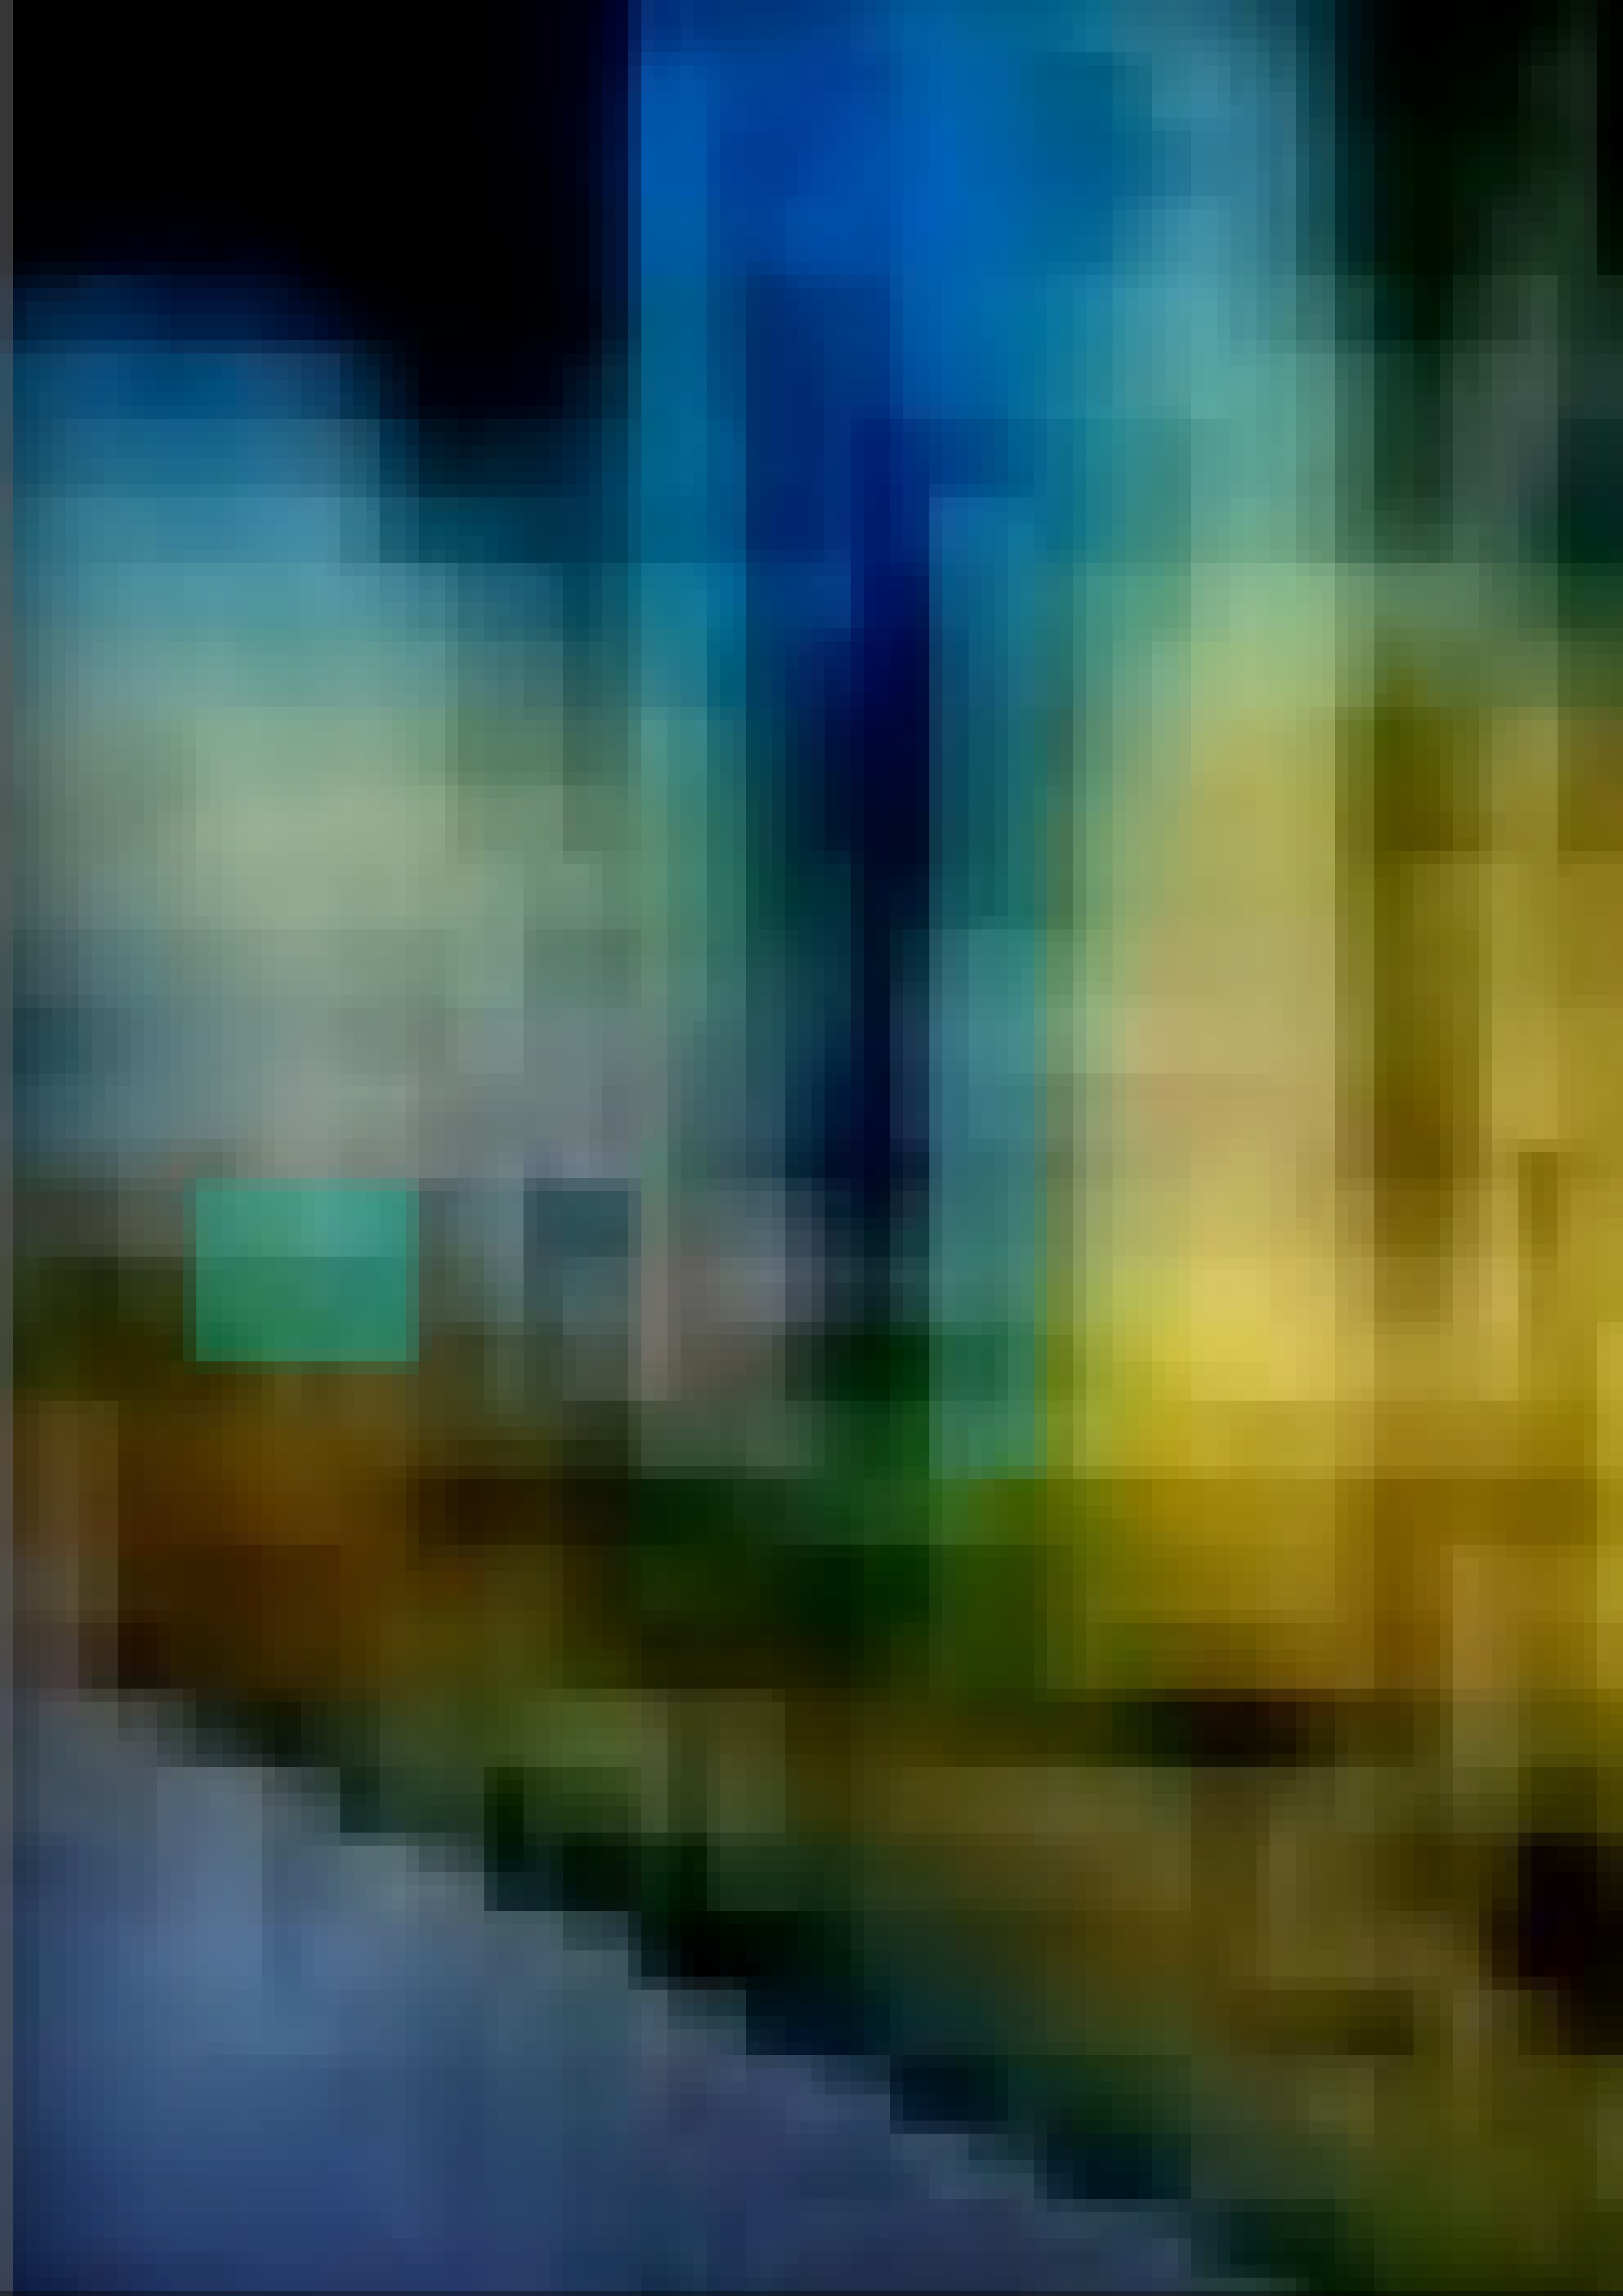
\includegraphics[width=0.4\textwidth]{Images/FrontCover.png}}
\end{figure}

\section{Motivation}
%There are some semi-interactive applications for image processing neural networks, such as style transfer. These applications are limited in the interactions they offer to the user. Often the only interactive part is the selection of the images that are fed into the algorithm. 
Using the representation of an environment a neural network has learned, to present the state of an environment to the player is still an nearly unexplored avenue. 
In this work I explore how neural networks can be used to create a unique interactive experiences, by using the output the neural representation of the network produces as the main information stream presented to the player.

\section{Scope}
what has been done, what pices constitute the work?
During the bachelor thesis the following things where developed:

\begin{itemize}
\item{Data generation environment}
\item{Data processing pipeline}
\item{Scene rendering neural network model and training pipeline}
\item{System to send network output in Unity}
\item{Merging of network output with unity rendered objects}
\item{Several exploratory prototypes}
\item{One extended Prototype (Maze game)}
\end{itemize}



\chapter{Background}
\section{Neural networks}
To give a better intuition for how neural networks are used in this project, a brief overview follows describing the components necessary to build a simple neural network. 

In brief a neural network is computational structure made up of multiple units called neurons.

\subsection{Neuron}
In its simple form a neuron can be defined as:
\begin{equation}
N_{\boldsymbol w, b}(\boldsymbol{x}) = \sigma\Bigg(b + \sum_{i=0}^{N}{\boldsymbol{w}_i \cdot \boldsymbol{x}_i}\Bigg)
\end{equation}
Where $\boldsymbol{x} \in \mathbb{R}^N$ is a vector containing all inputs and  $ \boldsymbol{w} \in \mathbb{R}^N$ a vector containing the neurons weights, $b \in \mathbb{R}$ is the bias, $N \in \mathbb{Z}$ is the number of inputs and $\sigma$ is a nonlinear function refereed to as the activation function of the neuron. This function is often set to be the rectified linear unit $ReLU(x) = \max(0, x)$.

Intuitively a neuron performs a weighted sum over its inputs adds a bias and applies an activation function to the result to calculate the final output.

\subsection{Multilayer network}
A neural network layer can be formed, multiple  the neurons are organized together in layers.

\section{Differential calculus}
Differential Calculus is an area of mathematics, that studies how a functions output changes with regard to tiny nudges to its inputs. 

\subsection{Univariate}
The derivative says how much the output of a function increases, at a specific point. It is defined as: 
\begin{equation}
\frac{df(x)}{dx} = \lim_{dx \to 0}\frac{f(x + dx) - f(x)}{dx}
\end{equation}
Intuitively this can be interpreted as the amount the output of the function changes when we increase the parameter to function by some tiny amount divided by how tiny that amount was. The $\lim_{dx \to 0}$ means, that we don't use a specific value for $dx$ but take the value the equation approaches when $dx$ approaches $0$, without $dx$ ever becomming $0$.

This means that the derivative can be used to find out how a function changes locally. If the derivative is positive and we increase the input to the function at the point the derivative was evaluated the output increases in size proportional to the magnitude of the derivative. The same logic applies when the derivative is negative.

%\begin{tikzpicture}
% \draw[->] (-2,0) -- (2,0) node[right] {x};
% \draw[->] (0,-1) -- (0,4) node[above] {y};
% \draw[scale=0.5,domain=-3:3,smooth,variable=\x,blue] plot ({\x}, {\x*\x});
%\end{tikzpicture}
%\begin{tikzpicture}
%\begin{axis}
%\addplot[color=red]{x*x};
%\tkzDefPoint(4,0){N}
%\end{axis}
%\end{tikzpicture}

\subsection{Multivariate}
The same can be applied to functions with multiple parameters:
\begin{equation}
\frac{\partial f(x_1, x_2)}{\partial x_1} = \lim_{\partial x_1 \to 0}\frac{f(x_1, x_2 + \partial x_1) - f(x_1, x_2)}{\partial x_1}
\end{equation}
\begin{equation}
\frac{\partial f(x_1, x_2)}{\partial x_2} = \lim_{\partial x_2 \to 0}\frac{f(x_1, x_2 + \partial x_2) - f(x_1, x_2)}{\partial x_2}
\end{equation}
Here each equation defines as how much the output of the function changes locally when the corresponding input parameter to the function varies.
The gradient of $f(x_1, x_2)$ is defined as:
\begin{equation}
\nabla f(x_1, x_2) = 
	\begin{bmatrix}
	\frac{\partial f(x_1, x_2)}{\partial x_1} \\[2mm]
	\frac{\partial f(x_1, x_2)}{\partial x_2}
	\end{bmatrix}
\end{equation}
This means the gradient contains all the information, of how a function varies

\subsection{Gradient decent}
Neu

\subsection{Chain rule}
\subsection{What more?}


\subsection{Backpropagation}
In practice neural networks are constructed as computation graphs. This means a the computations are defined by how edges connect to nodes, where the nodes correspond to operations to be performed.
Define computation graph, to enable reverse mode auto diff.

\subsection{GQN Network}
This work uses a simplefied implementation of the Generative Query Network \cite{gqn}.

In this work a network the architecture of GQN differs from the implementation used in the original paper. Here I use multilayer perceptron models for encoder and decoder without random latent variables. This circumvents the necessity of having to use the evidence lower bound as an optimization target.

This however prevents the network from taking into account the inputs given during inference to the same extent as in the original experiments described in the paper. The only meaningful considerations of the inputs of the network were found to be the coloring of the sky, floor and walls (when the latter view have the same color). In the original implementation the network can correctly infer more properties like object position, rotation and texture.

Because interesting use cases where found, that do not depend on this property of the GQN network no more effort was put into recreating the ability of the network to model different scenes.



\chapter{Workflow}
The first step was to create a working implementation of neural network, that is able to learn
out of what iteration flows was workflow composed \\
Research, Implementation, Variation

\section{Prototypes}
Multiple protoypes explored:

\subsection{Top down}
The goal of this prototype is, to test how well the network could be used to hide information in a simple top town navigation environment.
The idea is, that the network

Walking sim,
Object morphing
Maze,
Invisible Enemies



\chapter{Systems}
\section{Model}
Model in python

\subsection{Network} \label{Network}


\subsection{Saving and loading}
\section{Data Preprocessing}
\section{Inter process communication}
UDP sending of player position to python

Motion JPEG over UDP socket 

\section{Rendering}
In Unity the stream is decoded and rendered using custom Cg shaders. These shaders merges the network output stream with objects in the environment that are tagged to be visible in the combined render.

Cull objects if hidden from camera pos in unity environment

\section{Player interaction}
\paragraph{Laser}
player can shoot laser and destroy enemies

\paragraph{Smoke balls}
player can throw smoke balls which reveal invisible enemies and reveale the where the physical walls are in the smoke




\chapter{Further work}
In this section possible further applications based on the found data is discussed.

\section{Other directions with current state}
\subsection{Multiplayer Game}
2 Players are task to take observations of an environment that is rendered within the unity engine in a limited time. These observations  are now used as training data for a GQN. After training both player have to fight each other in this environment using the rendered output of the GQN.

\subsection{Merge output of multiple models}
\subsection{Blending of internal network state}
Lerp some parameters to network to create effect.

\section{Expand GQN capability}
GQN hard so not very good implementation. Variational metods, random ratent variables. Therefore only MLP.

\subsection{Generative model for modeling environment}
\subsection{Implement original GQN}
\subsection{Implement environment time step prediction}
\section{Expanded GQN directions}



\chapter{Reflection}
\section{Project}
The project has many flaws, list what did not work and how to remedy it.

\section{Workflow Evaluation}
Good, but more early on more strucktured exploration (especially automatic) for neural network parameter tweaks.

Dont scale up model to quickly -> higher res, rotation on x axis. this makes itteration time slower (longor training) and lead to many other problems cropping up, that force patchy solutions.





\chapter{Resources}
\section{Software}
\begin{itemize}
\item Unity3D
\item Git
\item Visual Studio
\item Python
\item PyCharm
\item Blender
\item Krita
\end{itemize}

\section{Unity packages}
\begin{itemize}
\item MK Toon Free (Toon shader) % & https://assetstore.unity.com/packages/vfx/shaders/mk-toon-free-68972 \\
\item Post Processing Stack % & https://assetstore.unity.com/packages/essentials/post-processing-stack-83912 \\
\item Universal Sound FX % & https://assetstore.unity.com/packages/audio/sound-fx/universal-sound-fx-17256 \\
\item Standard Assets % & https://assetstore.unity.com/packages/essentials/asset-packs/standard-assets-32351 \\
\item Ultimate Game Music Collection % & https://assetstore.unity.com/packages/audio/music/orchestral/ultimate-game-music-collection-37351 \\
\item Resonance Audio SDK for Unity v1.2.1 % & https://github.com/resonance-audio/resonance-audio-unity-sdk/releases \\
\end{itemize}

\section{Python packages}
\begin{tabular}{| r | l || r | l |}
\hline
absl-py             & 0.6.1 &
altgraph            & 0.16.1 \\ 
astor               & 0.7.1 &
certifi             & 2018.10.15 \\
Click               & 7.0 &
cycler              & 0.10.0 \\
Cython              & 0.29 &
dist-keras          & 0.2.1 \\
Flask               & 1.0.2 &
future              & 0.17.1 \\
gast                & 0.2.0 &
grpcio              & 1.12.1 \\
h5py                & 2.8.0 &
itsdangerous        & 1.1.0 \\
Jinja2              & 2.10 &
Keras               & 2.2.4 \\
Keras-Applications  & 1.0.6 &
Keras-Preprocessing & 1.0.5 \\
keyboard            & 0.13.2 &
kiwisolver          & 1.0.1 \\
macholib            & 1.11 &
Markdown            & 3.0.1 \\
MarkupSafe          & 1.0 &
matplotlib          & 3.0.1 \\
mkl-fft             & 1.0.6 &
mkl-random          & 1.0.1 \\
names               & 0.3.0 &
numpy               & 1.15.3 \\
olefile             & 0.46 &
pandas              & 0.23.4 \\
pefile              & 2018.8.8 &
Pillow              & 5.3.0 \\
pip                 & 10.0.1 &
protobuf            & 3.6.1 \\
pygame              & 1.9.4 &
PyInstaller         & 3.4 \\
pyparsing           & 2.2.2 &
PyQt5               & 5.11.2 \\
PyQt5-sip           & 4.19.12 &
python-dateutil     & 2.7.5 \\
pytz                & 2018.7 &
pywin32-ctypes      & 0.2.0 \\
PyYAML              & 3.13 &
scipy               & 1.1.0 \\
setuptools          & 39.1.0 &
six                 & 1.11.0 \\
tensorboard         & 1.11.0 &
tensorflow          & 1.11.0 \\
termcolor           & 1.1.0 &
Theano              & 1.0.3 \\
tornado             & 5.1.1 &
Werkzeug            & 0.14.1 \\
wheel               & 0.32.2 &
wincertstore        & 0.2 \\
\hline
\end{tabular}
\newpage

\section{Textures}
\begin{centering}
\begin{tabular}{l|l}
Texture & Source \\
\hline

\includegraphics[width=0.2\textwidth]{Images/BlackBorder.png} &  \\

\includegraphics[width=0.2\textwidth]{Images/BlackThickBorder.png} & 
\makecell[l]{Yannick Pawlis \\ Given on the 8.12.2018} \\
\hline
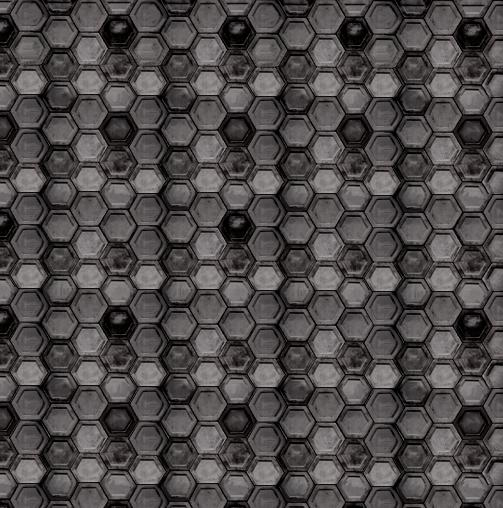
\includegraphics[width=0.2\textwidth]{Images/airbase_radar_panels.jpg} & 
\makecell[l]{Retrieved on the 8.12.2018 at \\ \linebreak https://opengameart.org/node/7254}
\end{tabular}
\end{centering}

\bibliographystyle{plain}
\bibliography{BachelorBooklet}

\listoffigures



\chapter*{Acknowledgments}
I like to thank Yannick Pawils for our daily insightful discussions and for his feedback which was a great guidance to me. \\
Also I like to thank my professor Thomas Bremer for the feedback and guidance he provided.\\
Furthermore I like to thank Susanne Brandhorst, Jules Pommier and Matthias Mayer.



\chapter*{Statement of Authorship}
I hereby declare that I am the sole author of this bachelor thesis and that I have not used any sources other than those listed in the bibliography- and resources section. I further declare that I have not submitted this thesis at any other institution in order to obtain a degree.
\begin{spacing}{5}
\null
\begin{spacing}{1}
\noindent
\dotfill \space \space \dotfill \\
(Place, Date) \hfill (Signature)\hfill \null
\end{spacing}
\end{spacing}



\newpage
\pagestyle{empty}
\centering
\vfill

\includegraphics[width=0.5\textwidth]{Images/logo_GD_black.jpg}
\vfill
\vspace*{-2cm}

\includegraphics[width=0.5\textwidth]{Images/logo_dehive.jpg}
\vfill

\includegraphics[width=0.5\textwidth]{Images/logo_htw.jpg}
\vfill



%\newpage
\blankpage
\blankpage
\blankpage

\begin{tikzpicture}[remember picture,overlay]
\node[inner sep=0pt] (background) at (current page.center) {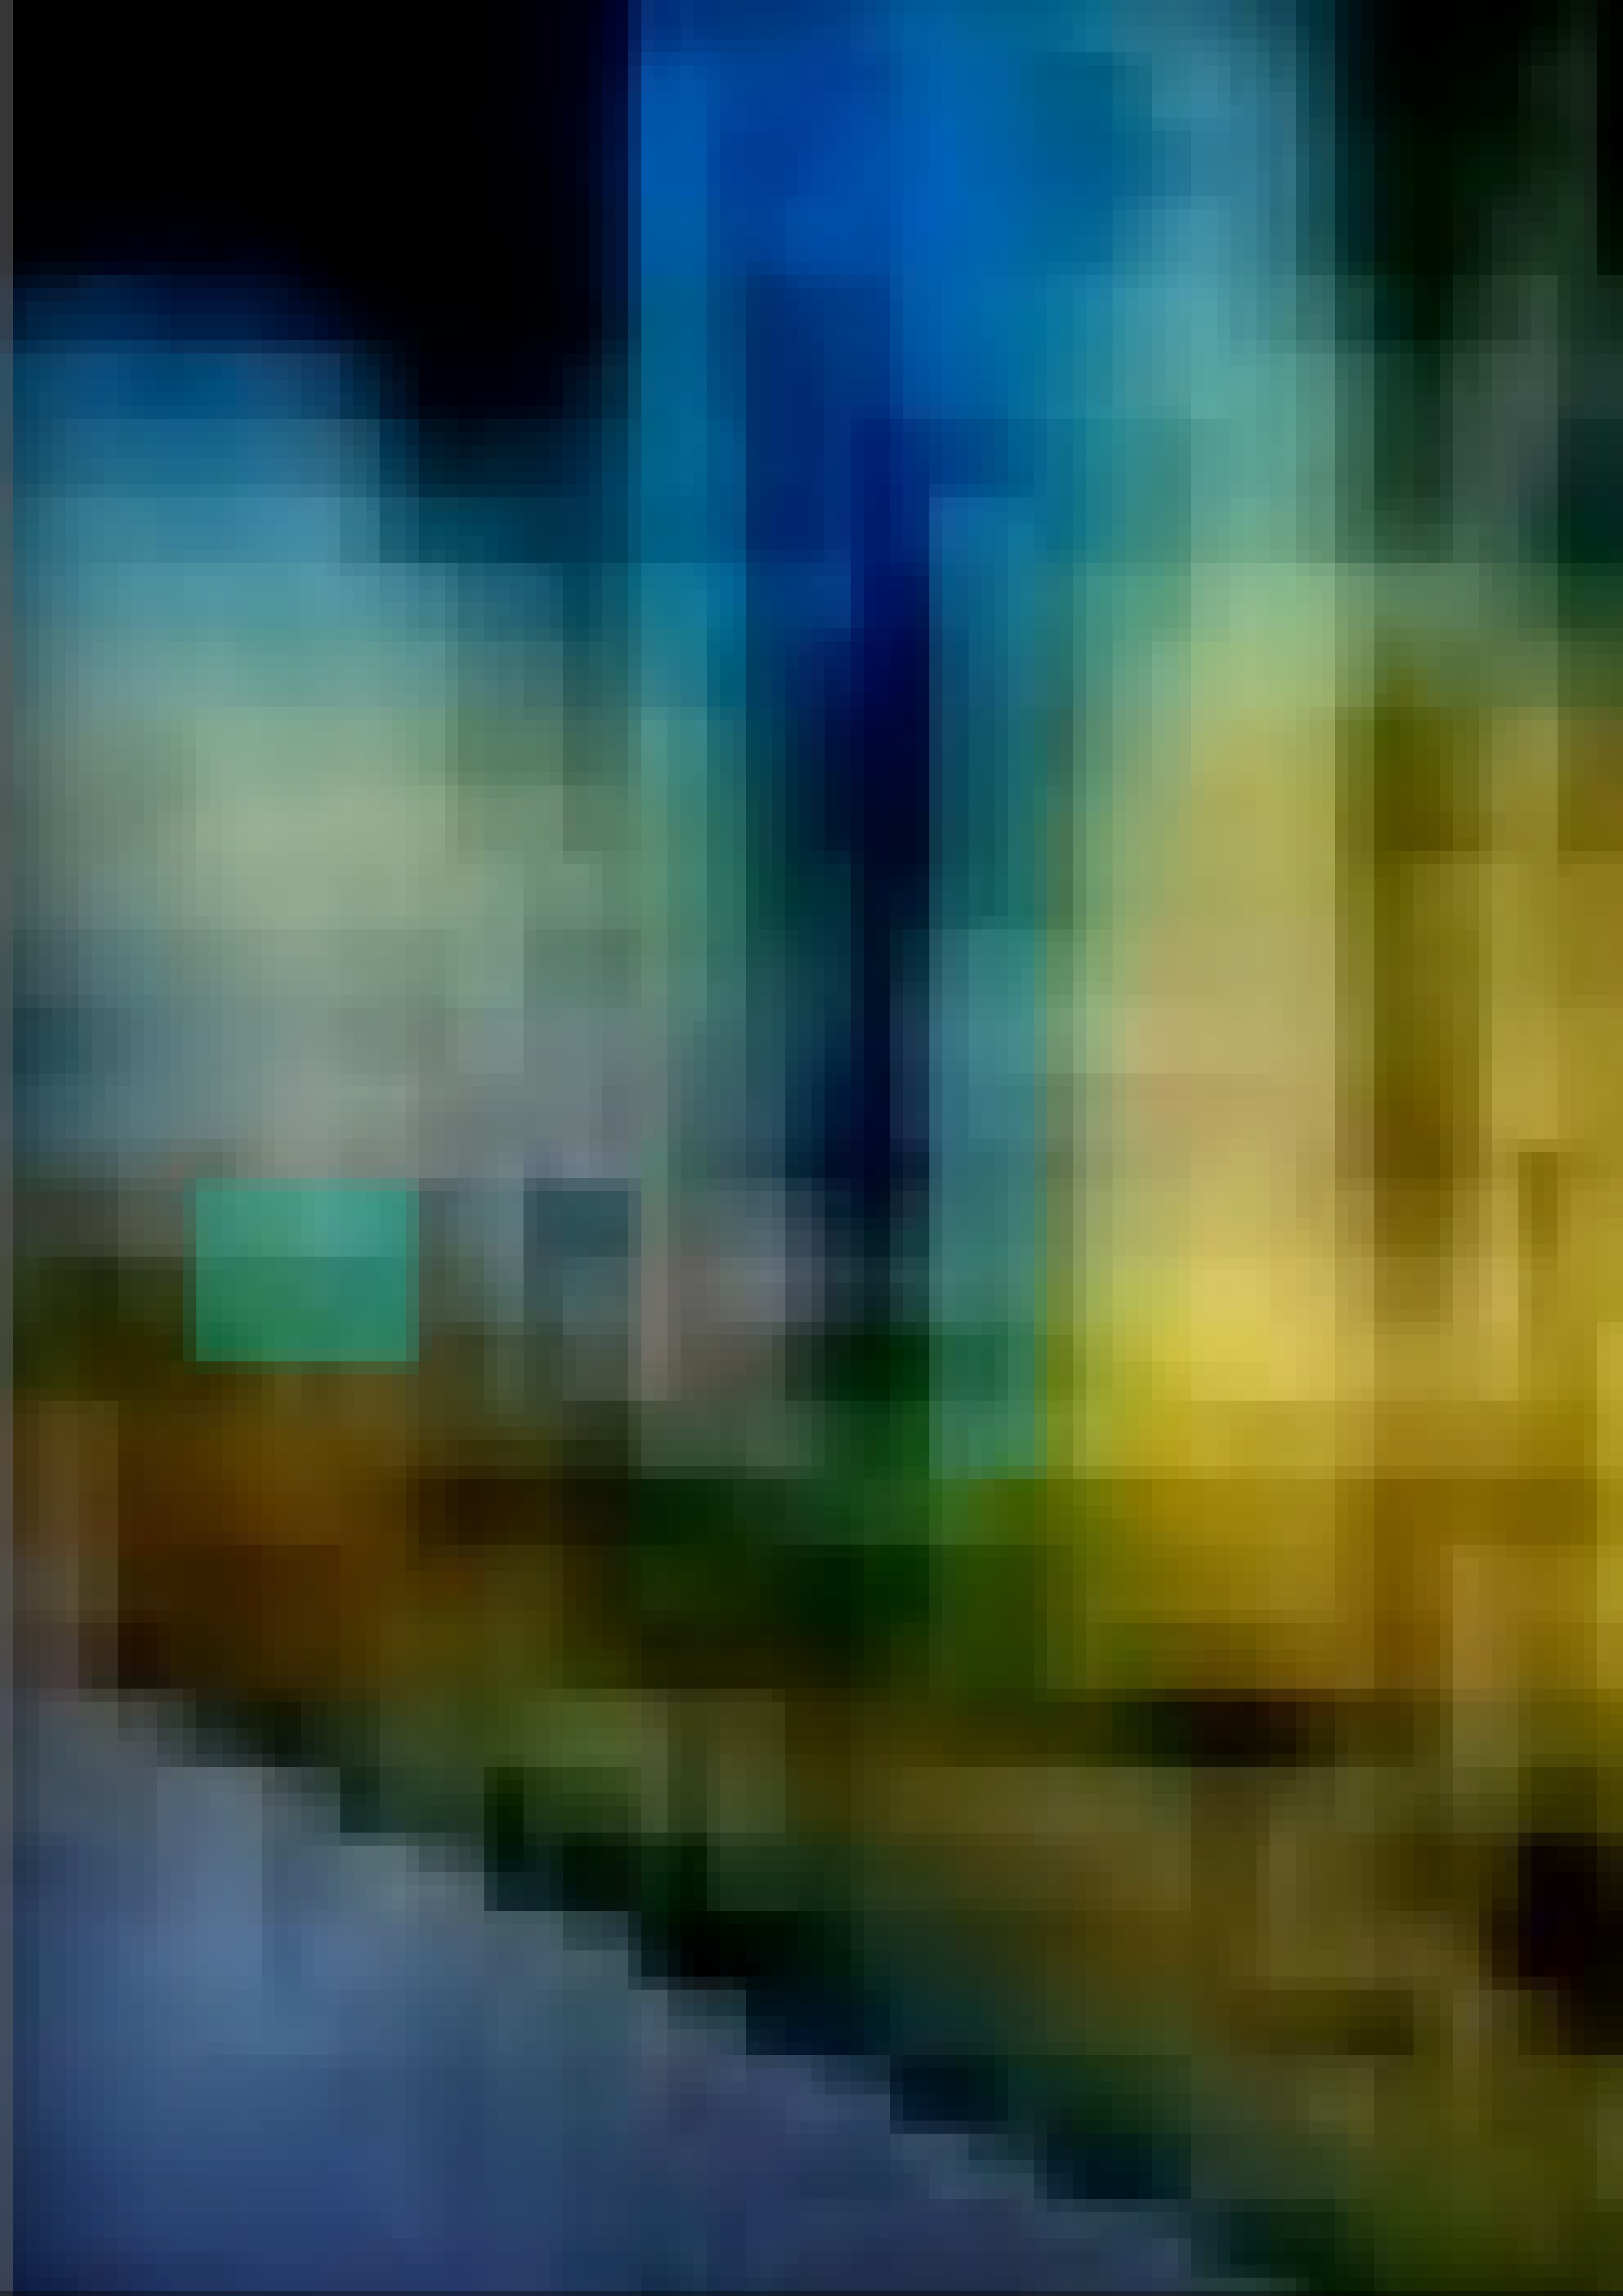
\includegraphics[width=\paperwidth]{Images/BackCover.png}};
\end{tikzpicture}

\end{document}